%%%%%%%%%%%%%%%%%%%%%%%%%%%%%%%%%%%%%%%%%%%%%%%%%%%%%%%%%%%%%%%%%%%%
%% I, the copyright holder of this work, release this work into the
%% public domain. This applies worldwide. In some countries this may
%% not be legally possible; if so: I grant anyone the right to use
%% this work for any purpose, without any conditions, unless such
%% conditions are required by law.
%%%%%%%%%%%%%%%%%%%%%%%%%%%%%%%%%%%%%%%%%%%%%%%%%%%%%%%%%%%%%%%%%%%%

\documentclass{beamer}  
\usetheme[faculty=fi]{fibeamer}
\usepackage[utf8]{inputenc}
\usepackage[
  main=english
]{babel}        %% typeset as follows:
%%
%%   \begin{otherlanguage}{czech}   ... \end{otherlanguage}
%%   \begin{otherlanguage}{slovak}  ... \end{otherlanguage}
%%
%% These macros specify information about the presentation
\title{Cache-Oblivious Priority Queue and Graph Algorithm Applications} %% that will be typeset on the
\author{Alexandru Furculita}
%% These additional packages are used within the document:
\usepackage{ragged2e}  % `\justifying` text
\usepackage{booktabs}  % Tables
\usepackage{tabularx}
\usepackage{tikz}      % Diagrams
\usetikzlibrary{calc, shapes, backgrounds}
\usepackage{amsmath, amssymb}
\usepackage{url}       % `\url`s
\usepackage{listings}  % Code listings
\frenchspacing
\begin{document}
  \frame{\maketitle}

  \AtBeginSection[]{% Print an outline at the beginning of sections
    \begin{frame}<beamer>
      \frametitle{Summary}
      \tableofcontents[currentsection]
    \end{frame}}

  \begin{darkframes}
    \section{Background and previous results}
    
    \subsection{I/O Model or external-memory model}
    \begin{frame}{I/O Model or external-memory model}
        \textbf{Memory architecture:}
        \begin{itemize}
            \item Internal memory of size \textit{\textbf{M}} and,
            \item Arbitrarily large external memory partitioned into blocks of size \textit{\textbf{B}}
        \end{itemize}
      	\bigskip
        \textbf{Efficiency measure:} the number of \textit{memory transfers}, the number of blocks transfered between the two levels of memory\\\bigskip
        \textbf{Limitations:}
        \begin{itemize}
            \item Parameters \textit{\textbf{B}} and \textit{\textbf{M}} must be known
            \item Does not handle multiple memory levels
            \item Does not handle dynamic \textbf{\textit{M}}
        \end{itemize}
    \end{frame}

    \subsection{Cache-oblivious model}
    \begin{frame}{Cache-oblivious model}
        \begin{itemize}
            \item Design and analyze algorithms in the I/O model, but without having the size of the memory and of the blocks as explicit parameters
            \item Analyze in the I/O model for optimal off-line cache replacement strategy: If the main memory is full, the ideal block in main memory is elected for replacement based on the future characteristics of the algorithm
        \end{itemize}
        \bigskip
        \textbf{Advantages:}
        \begin{itemize}
            \item Optimal on arbitrary level optimal on all levels
            \item Portability: \textbf{B} and \textbf{M} not hard-wired into algorithm
            \item Dynamic changing parameters
        \end{itemize}
    \end{frame}

	\subsection{Priority queues}
    \begin{frame}{Priority queues}
        \begin{itemize}
            \item Maintains a set of elements each with a priority (or key) under the operations insert, delete, and deletemin
        \end{itemize}
    \end{frame}
    
	\subsection{Priority queues in I/O Model}
    \begin{frame}{Priority queues in I/O Model}
        \begin{block}{Problem}
        Sort \textbf{\textit{N}} elements using an \(O(\log_B N)\) priority queue closer to optimal solution.
      \end{block}
      \bigskip
      The normal algorithms are a factor of \(\frac{\log_B N}{\log_\frac{M}{B} \frac{N}{B}}\) from optimal
    \end{frame}
    
	\subsection{I/O efficient graph algorithms}
    \begin{frame}{I/O efficient graph algorithms}
        \begin{block}{Problem}
        Develop I/O-efficient algorithms for:
        \begin{itemize}
        \item list ranking
        \item Euler Tour
        \item BFS
        \item DFS
        \end{itemize}
      \end{block}
    \end{frame}

	\section{Optimal Cache-Oblivious Priority queues}
    \subsection{Structure}
    \begin{frame}{Optimal Cache-Oblivious Priority queues}
    \framesubtitle{Levels}
    \begin{itemize}
    \item consists of \(\Theta(\log \log N)\) levels of size \(N\) to a constant \(c\)
    \item the size of a level corresponds to the number of elements that can be stored within it
    \end{itemize}
    \end{frame}

    \begin{frame}{Optimal Cache-Oblivious Priority queues}
    \framesubtitle{Buffers}
    A level consists of two levels:
    \begin{itemize}
    \item \textit{up buffer}: only one, can store up to \(X\) elements
    \item \textit{down buffers:} at most \(X^\frac{1}{3}\) such buffers, each containing between \(\frac{1}{2}X^\frac{2}{3}\) and \(2X^\frac{2}{3}\)
    \end{itemize}
    \bigskip
    Three invariants about the relationships between the elements if buffers of various levels are maintained:
    \begin{itemize}
    \item At level \textit{X}, elements are sorted among the down buffers
    \item At level \textit{X}, the elements in the down buffers have smaller keys than the elements in the up buffer
    \item The elements in the down buffers at level \textit{X} have smaller keys than the elements in the down buffers at the next higher level
    \end{itemize}
    \end{frame}

    \begin{frame}{Optimal Cache-Oblivious Priority queues}
    \framesubtitle{Layout}
         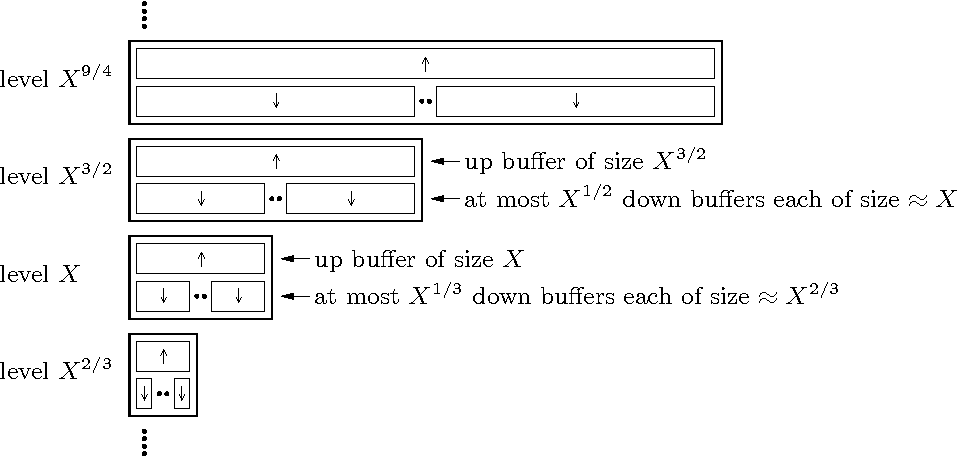
\includegraphics[width=\textwidth]{resources/queue}
    \end{frame}
    
    \subsection{Operations}

    \begin{frame}{Operations}
    \framesubtitle{Push}
    \begin{itemize}
    \item Inserts \textit{X} elements into level \(X^\frac{3}{2}\)
    \item Can be performed in \(O(X^\frac{1}{2} + \frac{X}{B}\log_\frac{M}{B} \frac{X}{B})\) memory transfers amortized
    \end{itemize}
    \end{frame}
    
    \begin{frame}{Push}
    \framesubtitle{Steps}
    To insert \textit{X} elements into level \(X^\frac{3}{2}\), we need to follow these steps:
    \begin{enumerate}
    \item Sort the \textit{X} elements
    \item Distribute the elements in the sorted list into the \(X^\frac{1}{2}\) down buffers of level \(X^\frac{3}{2}\) by scanning through the list and simultaneously visiting the down buffers in (linked) order.
    \item If the down buffer runs full, split the buffer
into two down buffers each containing X elements.
	\item If the level already had the
maximum number \(X^\frac{1}{2}\) of down buffers before the split, remove the last down buffer by inserting the less than \(2X\) elements  into the up buffer.
	\item If the up buffer runs full, all of these elements are recursively pushed into the next level up.
    \end{enumerate}
    \end{frame}

    \begin{frame}{Operations}
    \framesubtitle{Pull}
    \begin{itemize}
    \item Removes the \textit{X} elements with smallest keys from level \(X^\frac{3}{2}\) and returns them in sorted order
    \item Can be performed in \(O(1 + \frac{X}{B}\log_\frac{M}{B} \frac{X}{B})\) memory transfers amortized
    \end{itemize}
    \end{frame}

    \begin{frame}{Operations}
    \begin{block}{Total cost}
    A set of \textit{N} elements can be maintained in a linear-space cache-oblivious priority queue data structure supporting each insert, deletemin, and delete operation in \(O(\frac{1}{B}\log_\frac{M}{B} \frac{N}{B})\) amortized memory transfers and \(O(\log_2 N)\) amortized computation time.
    \end{block}
    \end{frame}
    
    \subsection{Graph algorithms}
    \begin{frame}{Graph algorithms applications and results}
    Using the cache oblivious priority queue, there can be developed cache oblivious algorithms for several graph problems that uses the same number of memory accesses as a cache-aware algorithm:
    \begin{itemize}
    \item The list ranking, the Euler Tour, BFS, DFS, and centroid decomposition problems on a \textit{V} node list can be solved in \(O(\frac{V}{B}\log_\frac{M}{B} \frac{V}{B})\) memory accesses
    \item The DFS or BFS tree of a directed graph can be computed in \(O((V + \frac{E}{B})\log_2 V + \frac{E}{B}\log_\frac{E}{B} \frac{E}{B})\) memory accesses.
    \item The BFS tree of an undirected graph can be computed cache-obliviously in \(O(N + \frac{E}{B}\log_\frac{M}{B} \frac{E}{B})\) memory accesses.
    \end{itemize}
    \end{frame}
    
    \begin{frame}{Graph algorithms}
    \framesubtitle{List ranking}
    \begin{block}{List ranking problem}
    	Given a linked list of \(V\) nodes, each with a pointer (edge) to the next node in the list, stored as an unordered sequence, determine the rank of each node \(v\), that is, the number of edges from \(v\) to the end of the list.
    \end{block}
    \end{frame}
    
    \begin{frame}{List ranking}
    \framesubtitle{Cache oblivious algorithm}
    The Cache oblivious algorithm for list ranking extends the existing I/O model algorithms by replacing the I/O model priority queues with cache oblivious priority queues.
    \bigskip
    \begin{block}{Chiang I/O Model algorithm}
    Find an independent set of \(O(V\)) nodes (nodes without edges
to each other), contract the edges incident to the nodes in
this set ("bridge out" the nodes in the independent set),
recursively rank the remaining list, and finally reintegrate the contracted nodes in the list (compute their rank).
    \end{block}
    \end{frame}
    
    \begin{frame}{List ranking}
    \framesubtitle{Chiang I/O Model algorithms adapted to Cache oblivious}
    The independent set algorithm of Chiang is
based on 3-coloring algorithms. It consists of the following steps:
    \begin{enumerate}
    \item the list is split into two sets consisting
of forward running segments (forward lists) and backward
running segments (backward lists). It is performed using a cache oblivious scanning.
	\item the nodes in the forward lists are colored red or blue by coloring the head nodes red and the other nodes alternatingly red and blue. The coloring is performed using a cache oblivious priority queue.
    \item the nodes in the backward lists are colored green and blue in a similar way, with the head nodes being colored green.
    \end{enumerate}
    \end{frame}
    
    \begin{frame}{List ranking}
    \framesubtitle{Chiang I/O Model algorithms adapted to Cache oblivious}
    As a result of these 3 steps, every node is colored with one color, except for the heads/tails which have two colors. 
    \bigskip
    
    By coloring a head/tail node red unless it was initially colored blue and green, in which case it is colored green, a 3-coloring is obtained.
    \end{frame}

    \begin{frame}[label=bibliography]{Bibliography}
      \begin{thebibliography}{9}
        \bibitem{demaine}
            Lars Arge, Michael A. Bender, Erik D. Demaine, Bryan Holland‐Minkley, and J. Ian Munro.
            \emph{An Optimal Cache‐Oblivious Priority Queue and Its Application to Graph Algorithms}.
            Available at \url{http://epubs.siam.org/doi/abs/10.1137/S0097539703428324}.
      \end{thebibliography}
    \end{frame}
  \end{darkframes}
\end{document}
